\documentclass[border=3pt]{standalone}
\usepackage[T1]{fontenc}
\usepackage[utf8]{inputenc}
\usepackage{lmodern}
\usepackage{amsmath,amssymb}
\usepackage{xcolor}
\usepackage{tikz}
\usepackage{fontawesome5}
\usepackage{ragged2e}
\usetikzlibrary{shapes,shapes.geometric,shapes.misc,arrows.meta,positioning,
                calc,fit,backgrounds,decorations.pathreplacing,
                decorations.markings,patterns,chains}
\usetikzlibrary{decorations.pathreplacing,decorations.markings}
\definecolor{primary}{HTML}{1A5276}
\definecolor{secondary}{HTML}{2E86C1}
\definecolor{accent}{HTML}{E74C3C}
\definecolor{lightbg}{HTML}{EBF5FB}
\definecolor{defbg}{HTML}{FDF2E9}
\definecolor{greenhl}{HTML}{27AE60}
\definecolor{purplehl}{HTML}{8E44AD}
\definecolor{goldhl}{HTML}{B7950B}
\definecolor{tealhl}{HTML}{117A65}
\definecolor{codebg}{HTML}{F4F6F7}
\definecolor{neutral}{HTML}{707B7C}
\definecolor{dom1}{HTML}{1F618D}
\definecolor{dom2}{HTML}{117864}
\definecolor{dom3}{HTML}{6C3483}
\definecolor{dom4}{HTML}{922B21}
\definecolor{dom5}{HTML}{B7950B}
% --- carried over from ccna.sty so figures match the book exactly
\tikzset{
  dev/.style={rounded corners=3pt, draw=#1, fill=#1!8, text=#1!45!black,
              line width=0.9pt, minimum width=1.45cm, minimum height=1.05cm,
              align=center, font=\scriptsize\bfseries, inner sep=2pt},
  wirestyle/.style={line width=0.9pt, neutral!75},
  xconn/.style={line width=0.9pt, neutral!75, dash pattern=on 2.5pt off 2pt},
}

\newcommand{\Rtr}[3]{\node[dev=dom3] (#1) at #2 {\faIcon{route}\\#3};}
\newcommand{\Sw}[3]{\node[dev=dom2] (#1) at #2 {\faIcon{sitemap}\\#3};}
\newcommand{\Msw}[3]{\node[dev=dom3] (#1) at #2 {\faIcon{layer-group}\\#3};}
\newcommand{\Host}[3]{\node[dev=neutral] (#1) at #2 {\faIcon{desktop}\\#3};}
\newcommand{\Lap}[3]{\node[dev=neutral] (#1) at #2 {\faIcon{laptop}\\#3};}
\newcommand{\Srv}[3]{\node[dev=dom1] (#1) at #2 {\faIcon{server}\\#3};}
\newcommand{\Ap}[3]{\node[dev=dom5] (#1) at #2 {\faIcon{wifi}\\#3};}
\newcommand{\Wlc}[3]{\node[dev=dom5] (#1) at #2 {\faIcon{broadcast-tower}\\#3};}
\newcommand{\Fw}[3]{\node[dev=dom4] (#1) at #2 {\faIcon{shield-alt}\\#3};}
\newcommand{\Cld}[3]{\node[dev=neutral] (#1) at #2 {\faIcon{cloud}\\#3};}
\newcommand{\Phone}[3]{\node[dev=dom5] (#1) at #2 {\faIcon{phone-alt}\\#3};}
\newcommand{\Prn}[3]{\node[dev=neutral] (#1) at #2 {\faIcon{print}\\#3};}

% A link. The optional argument takes tikz options (e.g. xconn for a
% trunk drawn dashed); the fourth argument labels the link.
\newcommand{\wire}[4][wirestyle]{%
  \draw[#1] (#2) -- node[font=\tiny, text=neutral!85!black, fill=white,
                          inner sep=1.2pt, midway] {#4} (#3);}
\newcommand{\plainwire}[3][wirestyle]{\draw[#1] (#2) -- (#3);}


\newenvironment{topology}[1][]
  {\begin{center}\begin{tikzpicture}[font=\scriptsize,#1]}
  {\end{tikzpicture}\end{center}}


\newcommand{\cmd}[1]{\texttt{\small #1}}
\newcommand{\term}[1]{\textbf{\textcolor{primary}{#1}}}
\newcommand{\chref}[1]{Chapter~\ref{ch:#1}}
\newcommand{\ccnafitw}[1]{#1}
\providecommand{\thefigure}{}
% --- progressive builds
\newcount\buildlevel \buildlevel=99
% \stepvis{n}{..} appears from level n onward; \steponly{n}{..} at
% level n alone, which is how a caption is swapped rather than
% accumulated as the build advances. \stepdim{n}{..} is the
% complement of \stepvis: it shows only BEFORE level n, so a
% pair of them draws an element faint and then solid. That keeps
% the canvas full from step 1, which matters for a figure whose
% shape is itself the lesson -- a five-rung ladder revealed one
% rung at a time leaves a void where the method should be.
\newcommand{\stepvis}[2]{\ifnum#1>\buildlevel\relax\else#2\fi}
\newcommand{\steponly}[2]{\ifnum#1=\buildlevel #2\fi}
\newcommand{\stepdim}[2]{\ifnum#1>\buildlevel #2\fi}
% Slide text does not hyphenate. A projected caption broken as
% ``uni-cast'' costs the reader a beat that print can afford and a
% lecture cannot, and the ragged edge it avoids is invisible at
% four metres anyway.
\hyphenpenalty=10000 \exhyphenpenalty=10000
\begin{document}
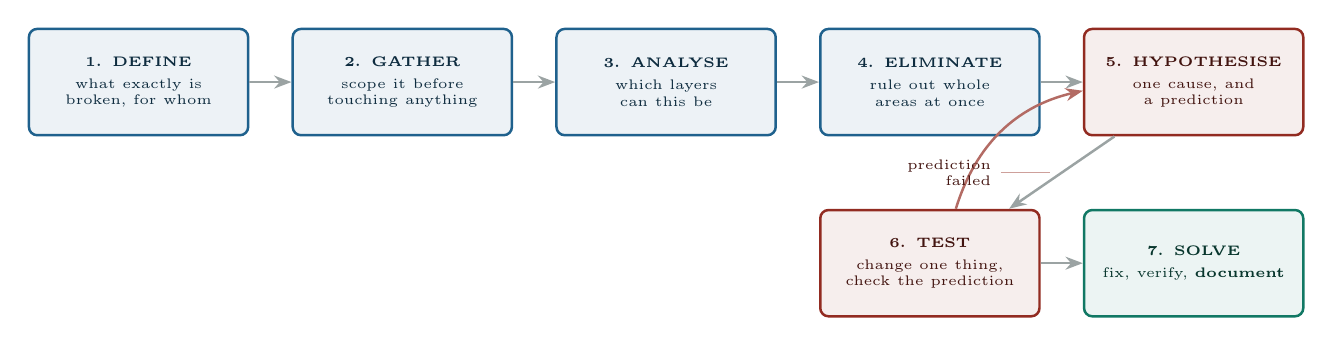
\begin{tikzpicture}[font=\scriptsize]
  \tikzset{
    st/.style={rounded corners=3pt, draw=#1, fill=#1!8, text=#1!45!black,
               line width=0.9pt, text width=2.55cm, align=center,
               minimum height=1.35cm, font=\tiny\bfseries},
    a/.style={-{Stealth[length=2.2mm]}, line width=0.9pt, neutral!70}}

  \node[st=dom1] (s1) at (0,0)     {1. DEFINE\\[2pt]\mdseries what exactly is
      broken, for whom};
  \node[st=dom1] (s2) at (3.35,0)  {2. GATHER\\[2pt]\mdseries scope it before
      touching anything};
  \node[st=dom1] (s3) at (6.7,0)   {3. ANALYSE\\[2pt]\mdseries which layers can
      this be};
  \node[st=dom1] (s4) at (10.05,0) {4. ELIMINATE\\[2pt]\mdseries rule out whole
      areas at once};
  \node[st=dom4] (s5) at (13.4,0)  {5. HYPOTHESISE\\[2pt]\mdseries one cause,
      and a prediction};

  \node[st=dom4] (s6) at (10.05,-2.3) {6. TEST\\[2pt]\mdseries change one thing,
      check the prediction};
  \node[st=dom2] (s7) at (13.4,-2.3)  {7. SOLVE\\[2pt]\mdseries fix, verify,
      \textbf{document}};

  \draw[a] (s1) -- (s2);  \draw[a] (s2) -- (s3);
  \draw[a] (s3) -- (s4);  \draw[a] (s4) -- (s5);
  \draw[a] (s5) -- (s6);
  \draw[a] (s6) -- (s7);

  % The label goes outside the arc, not inside it. Placed to the left of the
  % midway point it landed in the gap the arc encloses -- which is occupied by
  % the ELIMINATE box, so "prediction failed" printed across "rule out whole
  % areas at once" and neither could be read.
  \draw[a, dom4!70] (s6) to[bend left=30] (s5);
  % In the clear band between the two rows, immediately left of the arc's
  % bulge, with a leader so it cannot be read as labelling the grey 5-to-6
  % arrow on the other side.
  \node[font=\tiny, text=dom4!45!black, align=right, anchor=east] (pf)
      at (10.95,-1.15) {prediction\\failed};
  \draw[dom4!45, line width=0.6pt] (pf.east) -- ++(0.62,0);
\end{tikzpicture}
\end{document}
